\begin{exercice}[Calcul du ratio \ie]
	\begin{enumerate}
		\item Sur l'image suivante, au moyen d'une règle:

		\begin{enumerate}
			\item Tracer une ligne sur le début du Ti d'une percussion;
			\item Tracer une ligne sur le début du Te de cette percussion;
			\item Tracer une ligne sur le début du Ti de la percussion suivante;
			\item Mesurer la longueur du Ti et du Te;
		\end{enumerate}

		\item Diviser les deux chiffres par le plus petit des deux, afin
			de ramener à la forme $1:x$ ou $x:1$ \\(voir exemple plus bas).
	\end{enumerate}

	Que remarquez-vous ?

	\centering
	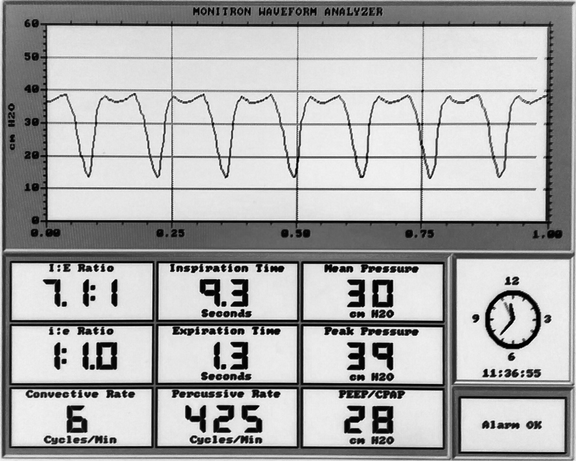
\includegraphics[height=6.5cm]{img/exr-ie-1}

\raggedright	\textbf{Exemple}
	\nopagebreak

\centering
	\begin{tikzpicture}[
				ann/.style={
					line width=1.4pt,
					dashed
				},
				fl/.style={
					<->,
					line width=1.3pt,
					shorten <=0.5mm,
					shorten >=0.5mm,
				},
				meas/.style={
					above=0mm,
					font=\bfseries,
				}
			]
		\node (IMG) {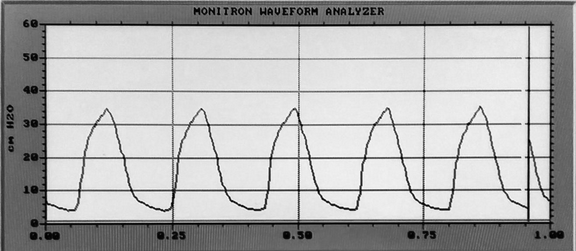
\includegraphics[height=4.8cm]{img/exr-ie-2}};
		\node at (3,.75) [matrix of math nodes, fill=white, rounded corners,
		opacity=0.87, draw=gray]{%
			i:e & =& 9:16\\
						 &=& \frac{9}{9}:\frac{16}{9}\\
						 &=& 1:1,78\\
			};

			\draw [ann](-2.15,-2) -- ++(0,4);
			\draw [ann](-1.6,-2) -- ++(0,4);
			\draw [ann](-.4,-2) -- ++(0,4);

			\draw [fl] (-2.15, 1) -- (-1.6, 1) node [meas, pos=0, anchor=
			east] {9 mm};
			\draw [fl] (-1.6, 1) -- (-0.4, 1) node [meas, pos=1, anchor=west] {16 mm};
	\end{tikzpicture}
\end{exercice}
